\documentclass[11pt,a4paper]{article}

\usepackage[T1]{fontenc}
\usepackage[utf8]{inputenc}
\usepackage{lmodern}
\usepackage[margin=2.5cm]{geometry}
\usepackage{amsmath,amssymb}
\usepackage{graphicx}
\usepackage{booktabs,array}
\usepackage[font=small,labelfont=bf]{caption}
\usepackage{xcolor}
\usepackage{listings}
\usepackage{url}
\usepackage[colorlinks=true,linkcolor=black,urlcolor=blue!50!black,citecolor=black]{hyperref}

\newcommand{\code}[1]{\path{#1}}          % inline code / file names
\newcommand{\vect}[1]{\mathbf{#1}}
\renewcommand{\arraystretch}{1.12}

\lstset{
  basicstyle=\ttfamily\small,
  breaklines=true,
  frame=single,
  rulecolor=\color{black!30},
  columns=fullflexible,
  keepspaces=true
}

\title{Technical Report}
\author{
	Palaniappan, Apurva \\ \small Team Member
	\and 
	Adrah, Michael \\ \small Team Member
	\and 
	Karmacharya, Harjit \\ \small Team Member
}
\date{\today}

\begin{document}
\maketitle

\section{Kinematic model}

\subsection{Robot and coordinate frames}

The SO-101 follower arm has five revolute joints that position and orient the tool, plus a gripper-jaw servo that does not move the tool frame. The kinematic chain therefore has $n=5$ joints and the tool pose is an element of $SE(3)$.

\begin{figure}[htbp]
  \centering
  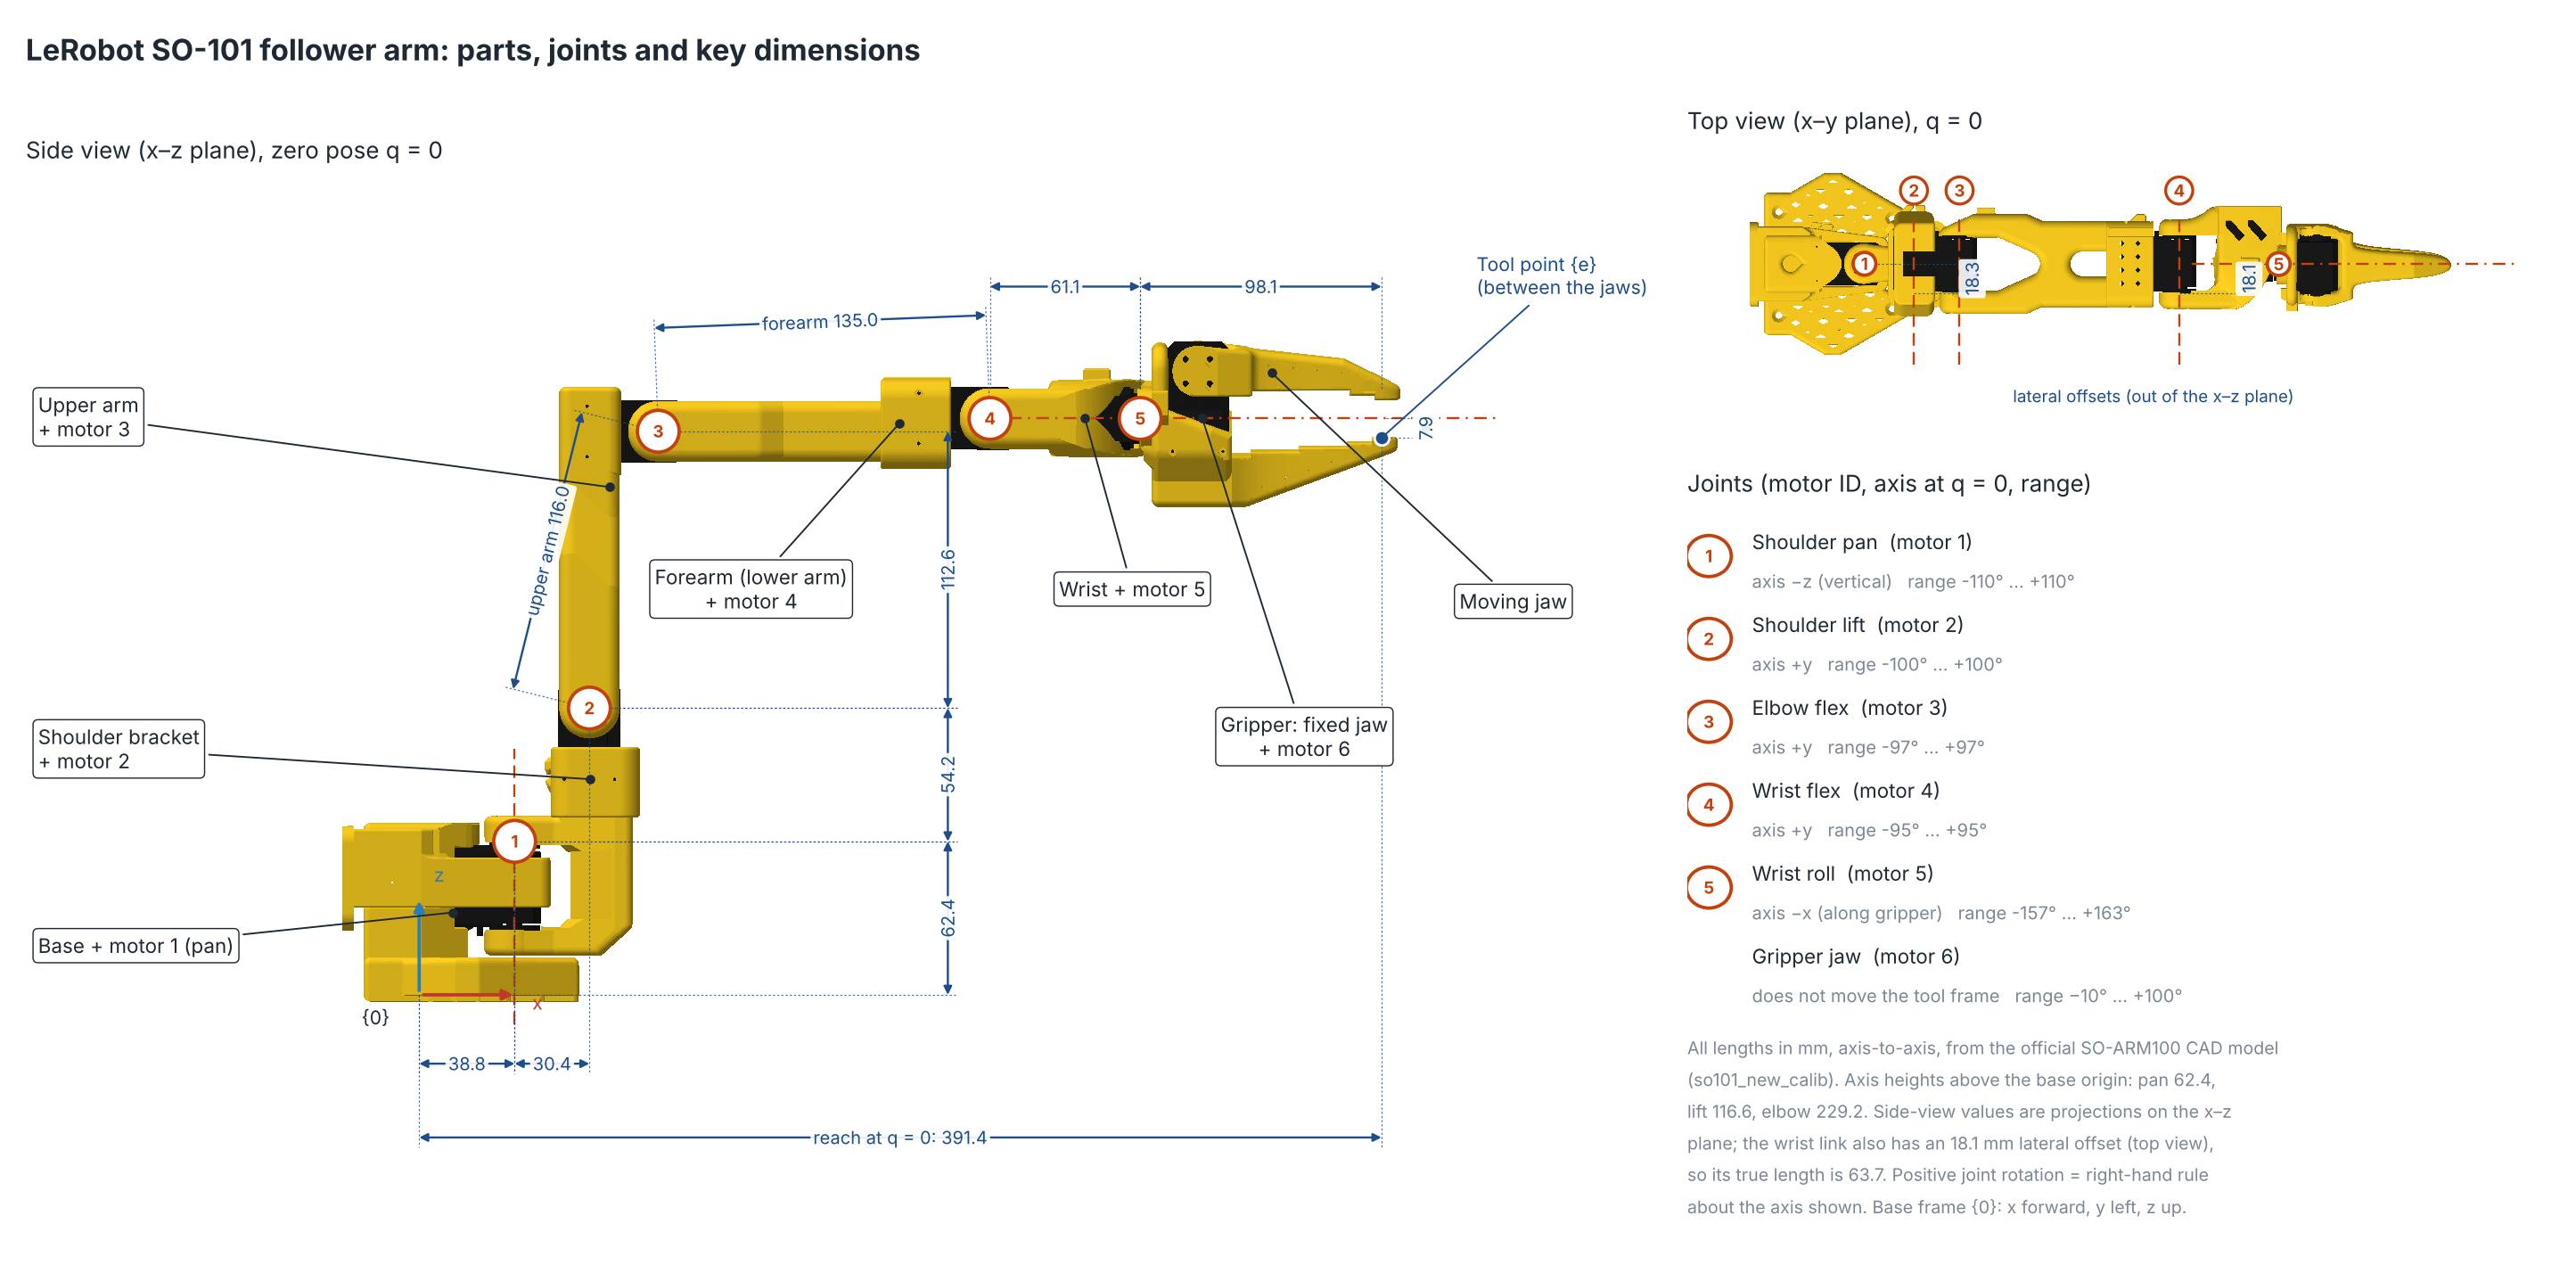
\includegraphics[width=\textwidth]{figures/so101_labeled_parts_dimensions.png}
  \caption{The SO-101 rendered from the CAD meshes at $q=0$: labelled parts, joint numbers and axes, and key dimensions in mm (side view projections; the top view shows the lateral offsets).}
  \label{fig:labelled}
\end{figure}

\paragraph{Frames.} Three kinds of frames are used:
\begin{itemize}
  \item \textbf{Base frame $\{0\}$}: origin at the origin of \code{base_link}, on the table plane at the centre of the base plate. $x$ points forward (towards the arm), $y$ to the left, $z$ up (right-handed).
  \item \textbf{End-effector frame $\{e\}$}: the URDF frame \code{gripper_frame_link}, located at the tool point between the two jaws. At $q=0$ its $z$-axis points forward along the gripper (the approach direction), its $y$-axis points left, and its $x$-axis points down, tilted by $2.79^\circ$ (see Section~\ref{sec:poe}).
  \item \textbf{Joint axes}: each joint $i$ rotates about a unit axis $w_i$ through a point $p_i$, both expressed in $\{0\}$ at the zero configuration. A positive joint angle is a right-hand rotation about $w_i$, the same sign convention as the URDF and the MuJoCo model, so joint values can be exchanged with MuJoCo without conversion.
\end{itemize}

\paragraph{Zero configuration.} $q=0$ is the ``new calibration'' zero of the official model: upper arm vertical, forearm horizontal pointing forward, gripper pointing forward (the ``L'' pose).

\paragraph{Joints.} Table~\ref{tab:joints} lists the five joints with their axes at $q=0$ and their limits.

\begin{table}[htbp]
  \centering
  \small
  \setlength{\tabcolsep}{4pt}
  \caption{Joint axes and limits of the SO-101 in the base frame at $q=0$ (source: official URDF).}
  \label{tab:joints}
  \begin{tabular}{@{}clllrr@{}}
    \toprule
    $i$ & Joint (motor ID) & Axis $w_i$ at $q=0$ & Point $p_i$ on axis [m] & Limits [rad] & Limits [deg] \\
    \midrule
    1 & shoulder\_pan (1)  & $(0,0,-1)$ & $(0.0388,\ 0,\ 0.0624)$       & $\pm 1.920$        & $\pm 110.0$ \\
    2 & shoulder\_lift (2) & $(0,1,0)$  & $(0.0692,\ -0.0183,\ 0.1166)$ & $\pm 1.745$        & $\pm 100.0$ \\
    3 & elbow\_flex (3)    & $(0,1,0)$  & $(0.0972,\ -0.0183,\ 0.2292)$ & $\pm 1.690$        & $\pm 96.8$  \\
    4 & wrist\_flex (4)    & $(0,1,0)$  & $(0.2321,\ -0.0183,\ 0.2344)$ & $\pm 1.658$        & $\pm 95.0$  \\
    5 & wrist\_roll (5)    & $(-1,0,0)$ & $(0.2932,\ -0.0002,\ 0.2344)$ & $-2.744\ldots 2.841$ & $-157.2\ldots 162.8$ \\
    \bottomrule
  \end{tabular}
\end{table}

\paragraph{Out-of-plane offset.} The shoulder-lift, elbow and wrist-flex axes are parallel and lie in a vertical plane 18.3~mm to the $-y$ side of the pan axis, because the shoulder-lift motor is mounted on the side of the shoulder bracket. The wrist link returns the roll axis to $y=-0.2$~mm, i.e.\ back to the centreline. This offset is invisible in a side view, but it is part of the geometry.

\begin{figure}[htbp]
  \centering
  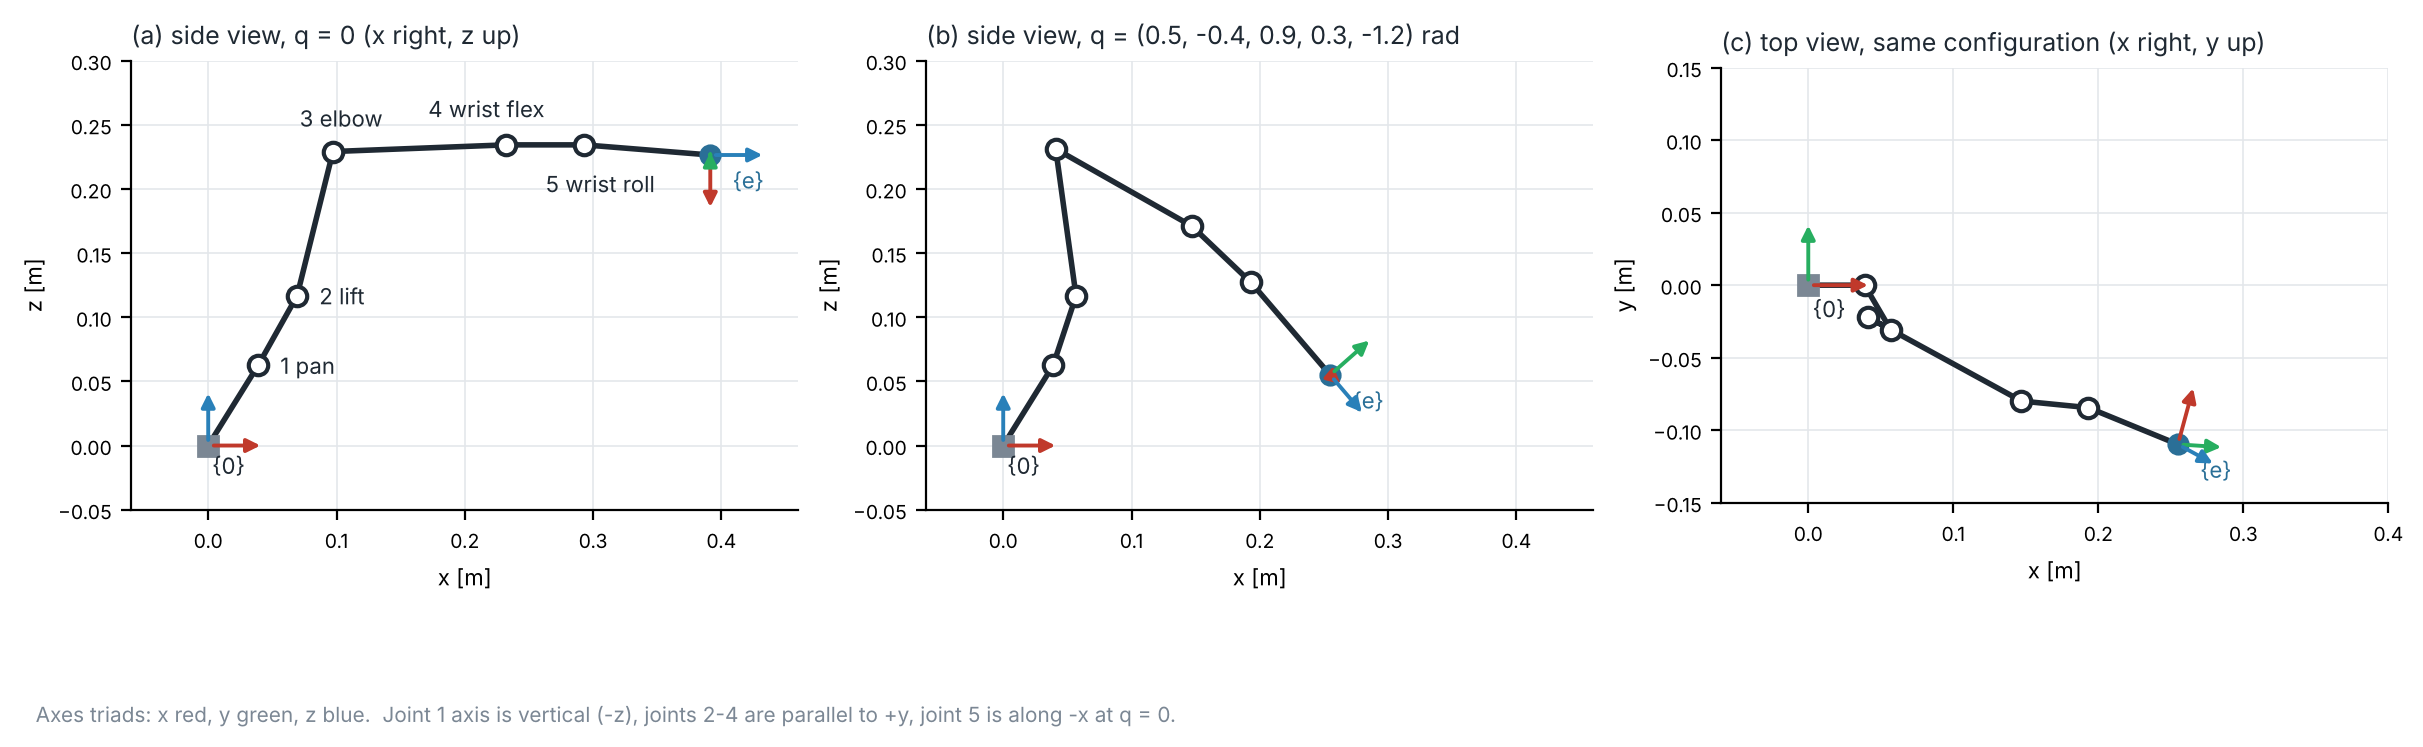
\includegraphics[width=\textwidth]{figures/so101_kinematic_diagram.png}
  \caption{Kinematic skeleton: (a) side view at $q=0$; (b) side view and (c) top view at $q=(0.5,-0.4,0.9,0.3,-1.2)$ rad. Frame triads: $x$ red, $y$ green, $z$ blue.}
  \label{fig:skeleton}
\end{figure}

\subsection{Product-of-Exponentials representation}
\label{sec:poe}

The arm is modelled with the Product-of-Exponentials (PoE) formulation in the space (base) frame, not with Denavit--Hartenberg (DH) parameters. PoE needs only the axis of every joint and the home pose of the end-effector, and all of these can be read directly from the CAD-derived model. A DH table would need extra offset parameters and a fixed tool transform to capture the 18.3~mm out-of-plane offset and the $2.79^\circ$ wrist tilt, and its frame assignment would not match the URDF frames. The screw axes also give the space Jacobian needed for inverse kinematics in the next phase without further derivation.

\paragraph{Screw axes.} Each revolute joint $i$ is described by the screw axis $S_i=(w_i,v_i)$, where $w_i$ is the unit rotation axis and $v_i=-w_i\times p_i$ is the linear part for a point $p_i$ on the axis, all in $\{0\}$ at $q=0$:

\begin{table}[htbp]
  \centering
  \small
  \caption{Screw axes $S_i=(w_i,v_i)$ of the SO-101 in the base frame.}
  \label{tab:screw}
  \begin{tabular}{@{}cllc@{}}
    \toprule
    $i$ & Joint & $w_i$ & $v_i$ [m] \\
    \midrule
    1 & shoulder\_pan  & $(0,0,-1)$ & $(0,\ 0.0388353,\ 0)$ \\
    2 & shoulder\_lift & $(0,1,0)$  & $(-0.1166,\ 0,\ 0.0692345)$ \\
    3 & elbow\_flex    & $(0,1,0)$  & $(-0.22917,\ 0,\ 0.0972345)$ \\
    4 & wrist\_flex    & $(0,1,0)$  & $(-0.23437,\ 0,\ 0.2321345)$ \\
    5 & wrist\_roll    & $(-1,0,0)$ & $(0,\ -0.23437,\ -0.0001778)$ \\
    \bottomrule
  \end{tabular}
\end{table}

\paragraph{Home pose.} The pose of $\{e\}$ in $\{0\}$ at $q=0$ is
\begin{equation}
  M = \begin{bmatrix}
    0 & 0 & 1 & 0.39136 \\
    \sin\alpha & \cos\alpha & 0 & -0.00001 \\
    -\cos\alpha & \sin\alpha & 0 & 0.22647 \\
    0 & 0 & 0 & 1
  \end{bmatrix}, \qquad \alpha = 0.0486795\ \text{rad} = 2.79^\circ .
\end{equation}
The tilt $\alpha$ is the CAD mounting offset of the wrist-roll servo. It is a real feature of the model and is kept, not rounded away: ignoring it would shift the orientation of $\{e\}$ by $2.79^\circ$.

\paragraph{How the parameters were obtained.} \code{tools/derive_poe_from_urdf.py} composes the fixed joint-to-joint transforms of the URDF at $q=0$, takes the $z$-axis of each joint frame as $w_i$ and its origin as $p_i$, and appends the fixed \code{gripper_frame_joint} transform to obtain $M$. The URDF stores angles with five digits (1.5708 instead of $\pi/2$), so any angle within $10^{-4}$ rad of a multiple of $\pi/2$ is snapped to it. Without this the axes would be tilted by about $10^{-5}$ rad. The only angle that is not a right angle, the 0.0486795~rad wrist-roll offset, is kept unchanged.

\subsection{Forward kinematics derivation}\label{sec:fk}

The end-effector pose for joint angles $q=(q_1,\ldots,q_5)$ is the product of five screw motions applied to the home pose:
\begin{equation}
  T_{0e}(q) = e^{[S_1]q_1}\, e^{[S_2]q_2}\, e^{[S_3]q_3}\, e^{[S_4]q_4}\, e^{[S_5]q_5}\, M .
  \label{eq:poe}
\end{equation}

\paragraph{Why this product.} With every joint at zero the tool pose is $M$. Rotating the last joint (wrist roll) by $q_5$ moves the tool rigidly about the fixed axis $S_5$, giving $e^{[S_5]q_5}M$. Rotating joint 4 by $q_4$ then carries the tool and axis 5 together about $S_4$, which is still the axis as it was at $q=0$ because it is expressed in the fixed space frame. Repeating this from the distal joint to the proximal one yields the product above, with joint 1 acting last on everything (Lynch and Park, \emph{Modern Robotics}, ch.~4~\cite{lynch}).

\paragraph{Matrix exponential of a revolute joint.} For a screw axis with $|w|=1$ and angle $\theta$, Rodrigues' formula gives the closed form that is implemented, with $[w]$ the skew-symmetric matrix of $w$:
\begin{equation}
  \begin{aligned}
    e^{[S]\theta} &= \begin{bmatrix} R & p \\ 0 & 1 \end{bmatrix}, \\
    R &= I + \sin\theta\,[w] + (1-\cos\theta)\,[w]^2, \\
    p &= \bigl(I\theta + (1-\cos\theta)[w] + (\theta-\sin\theta)[w]^2\bigr)\, v .
  \end{aligned}
\end{equation}
The tool position is $p_e(q)=T_{0e}[0{:}3,3]$ and its orientation is $R_e(q)=T_{0e}[0{:}3,0{:}3]\in SO(3)$.

\paragraph{Planar reduction as an analytic check.} With pan $=$ roll $=0$, joints 2--4 are parallel $y$-axes and the tool stays in the $x$--$z$ plane at constant $y$. Nesting the three rotations about the points $P_1,P_2,P_3$ on the axes gives, with $R_y(\theta)$ the rotation about $+y$ and the link vectors expressed at $q=0$:
\begin{equation}
  p_{xz} = P_1 + R_y(q_2)\Bigl[\ell_1 + R_y(q_3)\bigl[\ell_2 + R_y(q_4)\,\ell_3\bigr]\Bigr],
\end{equation}
\begin{equation*}
  \ell_1 = \begin{bmatrix}0.0280\\0.1126\end{bmatrix},\quad
  \ell_2 = \begin{bmatrix}0.1349\\0.0052\end{bmatrix},\quad
  \ell_3 = \begin{bmatrix}0.1592\\-0.0079\end{bmatrix}\ \text{m}.
\end{equation*}
The tool pitch is the sum $q_2+q_3+q_4$ applied to the home orientation. This closed form agrees with the PoE product to $1.7\times10^{-16}$~m over 200 random planar configurations, which checks the screw axes of joints 2--4 and the home pose independently of the exponential code.

\paragraph{Worked example.} For $q=(0.5,-0.4,0.9,0.3,-1.2)$ rad the product gives
\begin{equation}
  p_e = \begin{bmatrix}0.2549\\-0.1098\\0.0550\end{bmatrix}\ \text{m}, \qquad
  R_e = \begin{bmatrix}
    0.2555 & 0.7489 & 0.6114\\
    0.9413 & -0.0484 & -0.3340\\
    -0.2206 & 0.6609 & -0.7174
  \end{bmatrix}.
\end{equation}
MuJoCo returns the same position to within $4.5\times10^{-9}$~m. A sign check: a pure pan of $+45^\circ$ moves the tool from $(0.3914,\,0,\,0.2265)$ to $(0.2881,\,-0.2493,\,0.2265)$, i.e.\ clockwise seen from above, as expected for the axis $w_1=(0,0,-1)$.

\paragraph{Link to the Jacobian.} The same screw axes give the space Jacobian column by column, $J_i(q)=\mathrm{Ad}\bigl(e^{[S_1]q_1}\cdots e^{[S_{i-1}]q_{i-1}}\bigr)\,S_i$, which is what the inverse-kinematics phase will use.

\subsection{Implementation}

The forward kinematics is implemented in Python (NumPy) as a small package; the model constants are kept separate from the algorithm so that a calibrated parameter set could replace them without touching the code.

\begin{table}[htbp]
  \centering
  \small
  \caption{Files of the Phase~1 implementation.}
  \label{tab:files}
  \begin{tabular}{@{}p{0.36\textwidth}p{0.58\textwidth}@{}}
    \toprule
    File & Content \\
    \midrule
    \code{src/so101_model.py} & Joint names and limits, $w_i$, $p_i$, screw axes $S_i$, home pose $M$ \\
    \code{src/forward_kinematics.py} & \code{forward_kinematics(q)} returns the $4\times4$ pose; \code{forward_kinematics_pose(q)} returns (position, rotation); \code{within_joint_limits(q)} \\
    \code{tools/derive_poe_from_urdf.py} & Reproduces all model constants from the official URDF \\
    \code{tests/test_fk.py} & 12 unit tests, including a comparison with MuJoCo \\
    \code{simulation/validate_fk_mujoco.py} & FK versus MuJoCo over named and random configurations \\
    \bottomrule
  \end{tabular}
\end{table}

The interface takes the five arm joint angles in radians; a vector of any other length raises a \code{ValueError}, so the gripper angle cannot be passed by mistake.

\begin{lstlisting}[language=Python]
from src.forward_kinematics import forward_kinematics_pose

position, rotation = forward_kinematics_pose([0.5, -0.4, 0.9, 0.3, -1.2])  # rad
# position -> [ 0.2549, -0.1098, 0.0550 ] m,  rotation -> 3x3 matrix in SO(3)
\end{lstlisting}

The matrix exponential is evaluated with the closed-form Rodrigues expression of Section~\ref{sec:fk}, not with a general-purpose \code{expm}; the unit tests confirm that both agree to $10^{-12}$.

\subsection{Validation}\label{sec:valid}

The forward kinematics agrees with the official MuJoCo model to 15~nm in position and \mbox{$6.7\times10^{-8}$~rad} in orientation over 1000 random configurations, and the CAD link dimensions agree with measurements on the physical arm to within 4.6~mm. Three independent checks support this.

\paragraph{Unit tests.} The 12 tests in \code{tests/test_fk.py} all pass:

\begin{table}[htbp]
  \centering
  \small
  \caption{Unit tests of the forward kinematics.}
  \label{tab:tests}
  \begin{tabular}{@{}p{0.27\textwidth}p{0.67\textwidth}@{}}
    \toprule
    Check & What it verifies \\
    \midrule
    Zero pose & FK$(0)$ returns $M$ exactly \\
    $SO(3)$ and homogeneity & $RR^{\mathsf T}=I$, $\det R=1$, last row $(0,0,0,1)$ for 200 random configurations \\
    Screw axes & Unit-length $w_i$ and zero pitch ($w_i\cdot v_i=0$) \\
    Exponential & Closed form equals \code{scipy.linalg.expm} to $10^{-12}$ \\
    Pure pan & Tool height and distance to the pan axis stay constant \\
    Pure roll & Tool moves on a circle of radius 7.9~mm about the roll axis \\
    Planar motion & With pan $=$ roll $=0$ the tool stays in the $x$--$z$ plane \\
    Shoulder lift & Distance from the lift axis to the tool is independent of $q_2$ \\
    Interface & Pose and matrix outputs are consistent; a wrong-length input raises \\
    Joint limits & Helper accepts $q=0$ and rejects a pan of 2.5~rad \\
    MuJoCo match & 100 random configurations within $10^{-5}$~m and $10^{-5}$~rad \\
    \bottomrule
  \end{tabular}
\end{table}

\paragraph{Comparison with MuJoCo.} \code{simulation/validate_fk_mujoco.py} sets the joint angles in the official MuJoCo model, runs its kinematics and reads the pose of the \code{gripperframe} site. MuJoCo's world frame coincides with $\{0\}$. Nine named configurations (zero pose, single-joint moves, a folded pose, mixed poses) and 1000 random configurations drawn uniformly inside the joint limits (seed 0) were compared:

\begin{table}[htbp]
  \centering
  \small
  \caption{FK versus MuJoCo. The nine named configurations are within $1.0\times10^{-8}$~m and $4.2\times10^{-8}$~rad.}
  \label{tab:mujoco}
  \begin{tabular}{@{}lccc@{}}
    \toprule
    Metric (1000 random configurations) & Max & Mean & RMS \\
    \midrule
    Position error [m]        & $1.5\times10^{-8}$ & $7.9\times10^{-9}$ & $9.1\times10^{-9}$ \\
    Orientation error [rad]   & $6.7\times10^{-8}$ & $3.5\times10^{-8}$ & $3.8\times10^{-8}$ \\
    \bottomrule
  \end{tabular}
\end{table}

\begin{figure}[htbp]
  \centering
  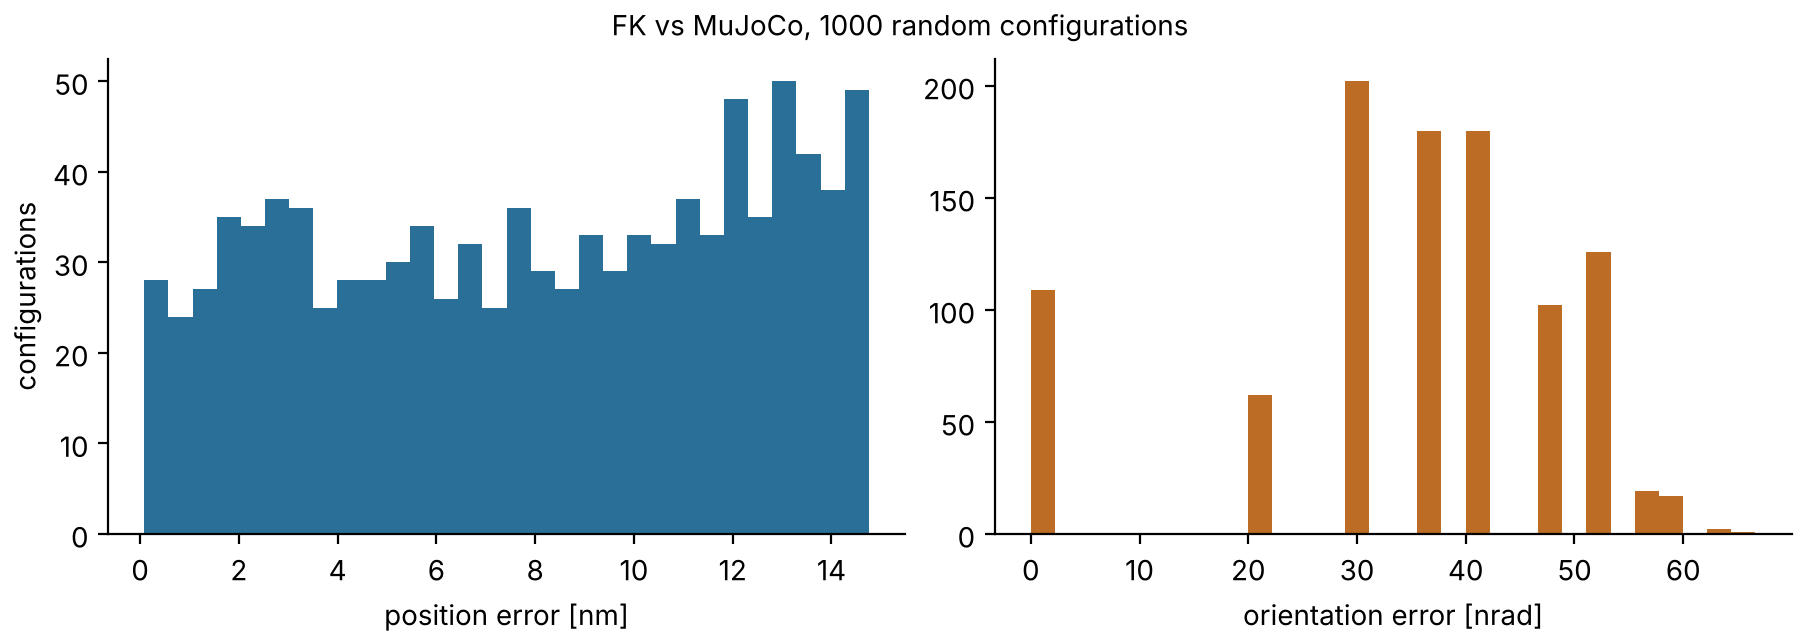
\includegraphics[width=0.92\textwidth]{figures/fk_validation_errors.png}
  \caption{Distribution of the FK error against MuJoCo (position in nm, orientation in nrad).}
  \label{fig:errors}
\end{figure}

The residual is at the level of floating-point and URDF angle rounding, so the implementation, the axis signs and the frame definitions are correct. One convention difference had to be handled: MuJoCo's \code{gripperframe} site and the URDF \code{gripper_frame_link} share the same origin but differ by a fixed rotation of $-90^\circ$ about the tool $y$-axis. This offset is constant to $10^{-14}$ over 500 random configurations. The model uses the URDF frame, which is the one LeRobot's own kinematics targets, and the validation script compensates the offset and also prints the raw $90^\circ$ difference.

\paragraph{Comparison with the physical arm.} Because MuJoCo and the model both derive from the same CAD numbers, the comparison above does not show that the real arm matches the CAD. The link dimensions were therefore measured on the arm and compared with the model:

\begin{table}[htbp]
  \centering
  \small
  \caption{Link dimensions: CAD model versus measurement on the arm.}
  \label{tab:measured}
  \begin{tabular}{@{}lccc@{}}
    \toprule
    Dimension & CAD [mm] & Measured [mm] & Difference [mm] \\
    \midrule
    Pan axis $\to$ lift axis, forward          & 30.4  & 35    & $+4.6$ \\
    Pan axis $\to$ lift axis, up               & 54.2  & 55    & $+0.8$ \\
    Upper arm (lift $\to$ elbow axis)          & 116.0 & 114.0 & $-2.0$ \\
    Forearm (elbow $\to$ wrist-flex axis)      & 135.0 & 139.0 & $+4.0$ \\
    Wrist (wrist-flex $\to$ roll axis)         & 63.7  & 64    & $+0.3$ \\
    Roll axis $\to$ tool point                 & 98.4  & 99    & $+0.6$ \\
    \bottomrule
  \end{tabular}
\end{table}

All differences are within 5~mm. The 4.6~mm difference of the first row is consistent with a straight-line horizontal measurement, which includes the 18.3~mm sideways offset:
\[ \sqrt{30.4^2+18.3^2}=35.5\ \text{mm}. \]
The remaining differences of $-2.0$ and $+4.0$~mm are of the size expected from reading the centres of servo horns on printed parts. The CAD values were kept as the nominal model, since a hand measurement is not more accurate than the CAD.

\subsection{Limitations and discussion}

The model is a rigid-body kinematic model of the CAD geometry, accurate to a few millimetres on the real arm. Its main limitations are:
\begin{itemize}
  \item \textbf{Same-source validation.} The MuJoCo comparison shares its geometry with the model, so it validates the implementation but not the hardware. The physical check in Section~\ref{sec:valid} covers link lengths only; a tool-position check at known table positions remains to be done in the hardware phase.
  \item \textbf{Not modelled.} Servo backlash, gear compliance, printed-part tolerances and calibration offsets are ignored. An angular error of $0.5^\circ$ at the shoulder-lift joint moves the tool by about 3~mm at the 0.34~m distance between that axis and the tool, which is the same size as the dimension differences in Table~\ref{tab:measured}.
  \item \textbf{Joint units and limits.} The LeRobot software reports joint values in its own units and calibration. A conversion to radians with the correct sign and zero offset is needed before commanding the arm, and the limits in Table~\ref{tab:joints} come from the simulation model and must be checked against the real arm.
  \item \textbf{Five degrees of freedom.} Five joints cannot reach an arbitrary pose in $SE(3)$: the reachable tool poses form a five-dimensional set, so the inverse-kinematics phase must treat position and orientation targets accordingly. The gripper jaw is not part of the chain and does not change the tool frame.
  \item \textbf{Tool frame.} $\{e\}$ is the URDF \code{gripper_frame_link}, placed at the middle of the jaws and 7.9~mm off the roll axis. A different tool point would only change $M$, not the screw axes.
\end{itemize}

\begin{thebibliography}{9}
  \bibitem{lynch} K.~M. Lynch and F.~C. Park, \emph{Modern Robotics: Mechanics, Planning, and Control}, Cambridge University Press, 2017, ch.~3--4 (screw axes, product of exponentials).
  \bibitem{sorarm} TheRobotStudio, SO-ARM100 repository, \code{Simulation/SO101}: \code{so101_new_calib.urdf}, \code{so101_new_calib.xml} and meshes. \url{https://github.com/TheRobotStudio/SO-ARM100/tree/main/Simulation/SO101}
  \bibitem{mujoco} E.~Todorov, T.~Erez and Y.~Tassa, ``MuJoCo: A physics engine for model-based control,'' \emph{IEEE/RSJ International Conference on Intelligent Robots and Systems (IROS)}, 2012.
\end{thebibliography}

\nocite{sorarm,mujoco}

\end{document}
